%--------------------------------------
% Spécifications du chat Felix - Camix
%
% IHM
%--------------------------------------

\section{Interface homme-machine}
\label{sec:ihm}

\subsection{Interface homme-machine de Felix}
\label{sec:ihm:felix}

La figure~\ref{sec:ihm:felix:fig} présente l'interface homme-machine (IHM) du client chat Felix.

\begin{figure}[h!]
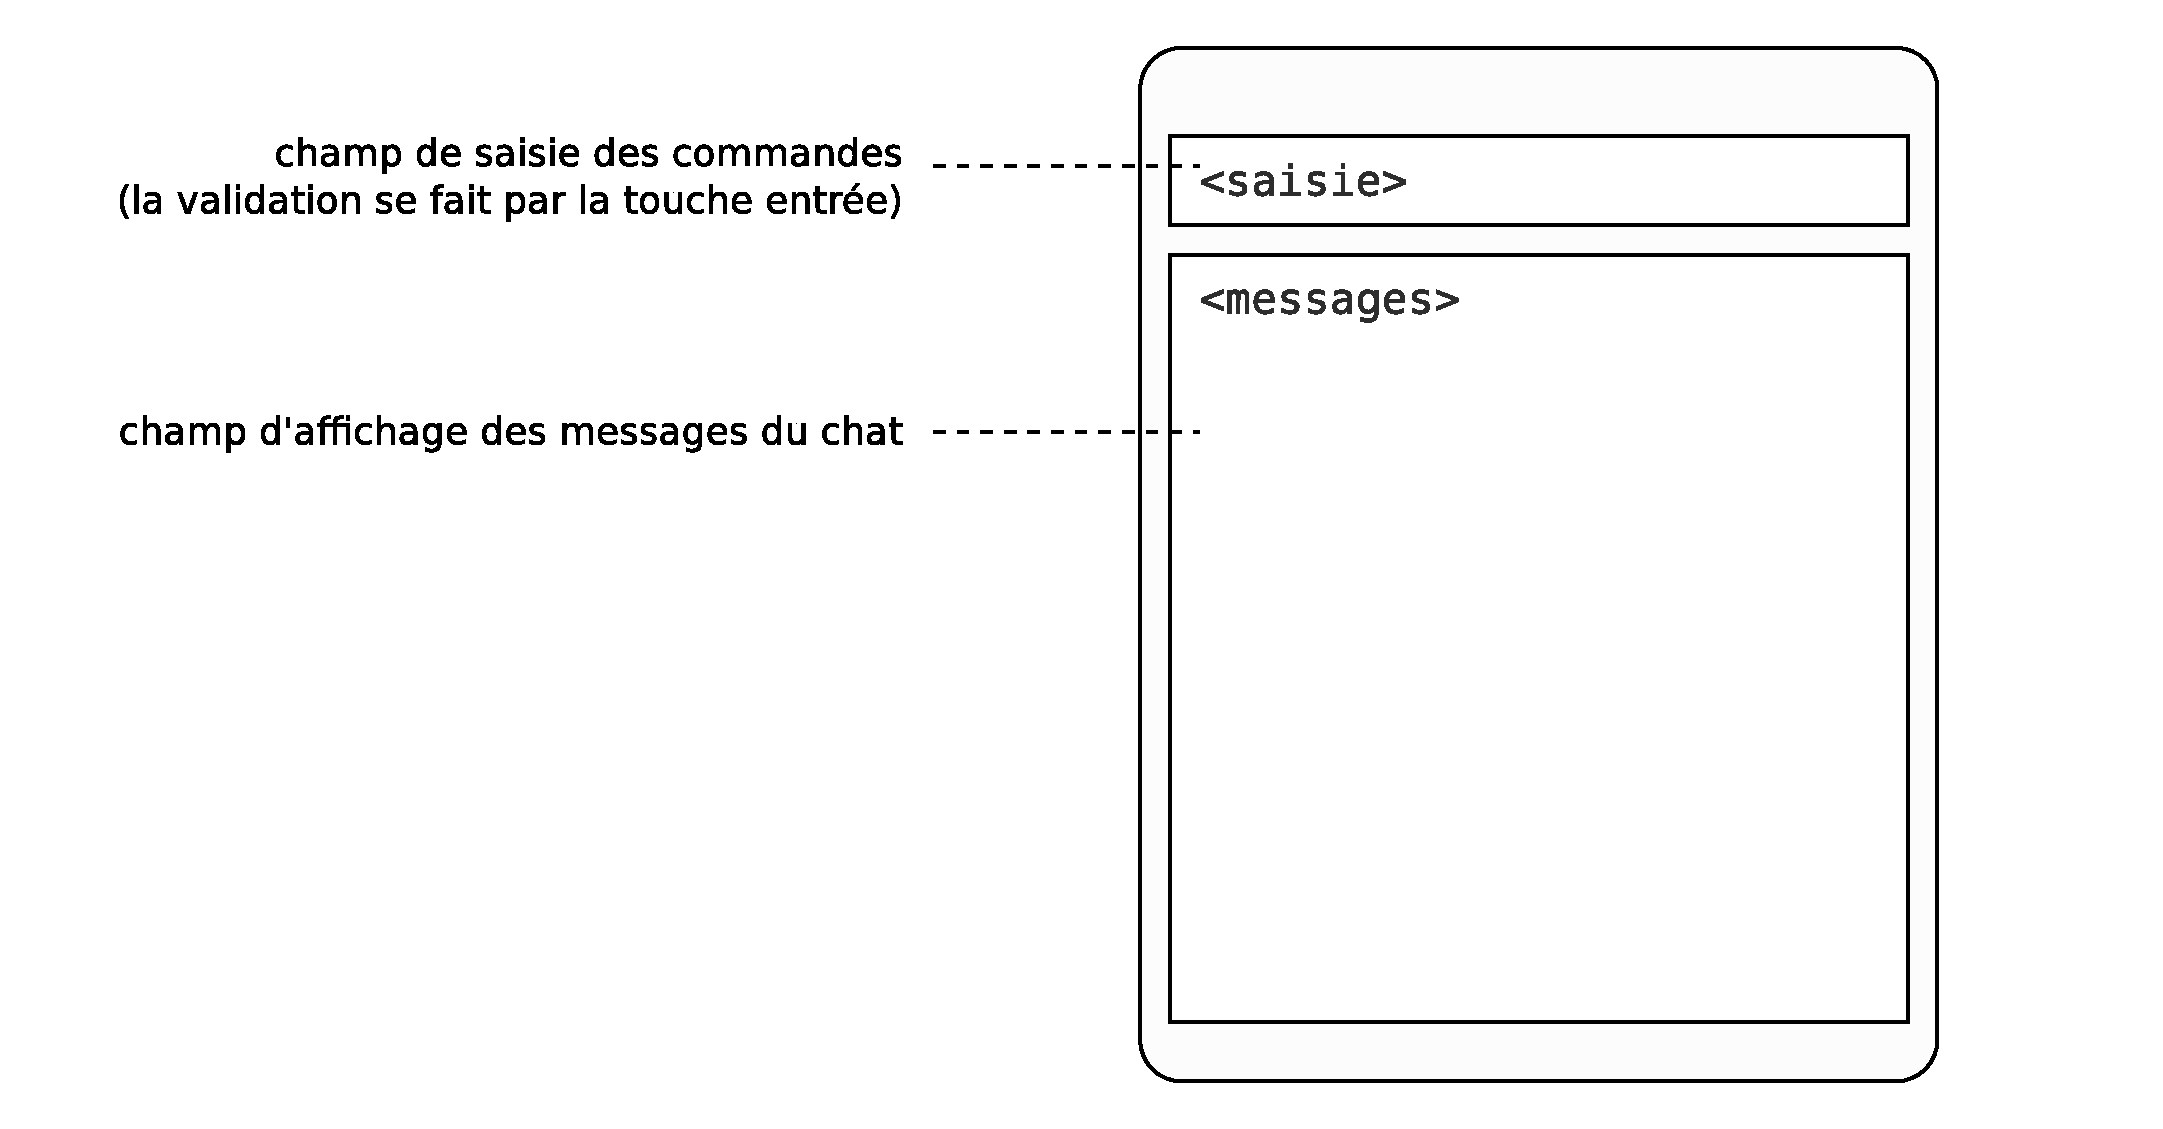
\includegraphics[width=\linewidth]{../img/Chat_IHM.eps}
\caption{IHM du client chat Felix : vue chat.}
\label{sec:ihm:felix:fig}
\end{figure}

\subsection{Protocole de communication client/serveur}
\label{sec:ihm:protocole}

Pour utiliser les différentes fonctionnalités du chat un protocole est à la disposition des utilisateurs.
Ce protocole définit un ensemble de commandes que peut invoquer un utilisateur.

\medskip
Le tableau~\ref{sec:cu:protocole:commandes} énumère les commandes disponibles dans le chat.

\medskip
\begin{table}[h!]
\renewcommand{\arraystretch}{1.3}
\begin{center}
\begin{tabular}{|l|l|}
\hline
   /n \textit{surnom} & Changer de surnom. \\
   /a \textit{nom du canal} & Créer un canal de discussion. \\
   /r \textit{nom du canal} & Supprimer un canal de discussion. \\
   /c \textit{nom du canal} & Changer de canal de discussion. \\
   /l & Afficher la liste des canaux de discussion. \\
   /? & Afficher ses informations personnelles. \\
   /h & Afficher l'aide sur les commandes du chat. \\
\hline
\end{tabular}
\caption{Liste des commandes du chat.}
\label{sec:cu:protocole:commandes}
\end{center}
\end{table}

\subsection{Messages textuels}
\label{sec:ihm:message}

L'utilisation du chat prévoit des messages communiqués aux utilisateurs par le serveur.
Les listings~\ref{sec:ihm:message:arrivee}, page~\pageref{sec:ihm:message:arrivee}, à \ref{sec:ihm:message:suppressionplacepublique}, page~\pageref{sec:ihm:message:suppressionplacepublique}, spécifient ces différents messages.

\bigskip
\begin{lstlisting}[caption={\normalsize{Message d'arrivée d'un utilisateur dans le chat {\footnotesize(à destination de la place publique)}.}},label={sec:ihm:message:arrivee}]
* Un nouvel utilisateur est dans le chat (place publique).
\end{lstlisting}

\medskip
\begin{lstlisting}[caption={\normalsize{Message d'accueil dans le chat.}},label={sec:ihm:message:accueil}]
* Taper /h pour avoir de l'aide sur les commandes du chat.
\end{lstlisting}

\medskip
\begin{lstlisting}[caption={\normalsize{Message d'aide sur les commandes du chat.}},label={sec:ihm:message:aide}]
* Commandes disponibles : 
   /n : changer de surnom ;
   /c : changer de canal ;
   /l : afficher les canaux ;
   /a : créer un canal ;
   /r : supprimer un canal ;
   /? : afficher ses informations ;
   /h : afficher l'aide.
\end{lstlisting}

\medskip
\begin{lstlisting}[caption={\normalsize{Exemple de message transmis dans le chat.}},label={sec:ihm:message:message}]
utilisateur_x > Hello World !

Remarque : Un message est préfixé par le surnom de l'émetteur suivi de '>'.
\end{lstlisting}

\medskip
\begin{lstlisting}[caption={\normalsize{Exemple de message de changement de surnom d'un utilisateur.}},label={sec:ihm:message:surnom}]
* utilisateur_x devient utilisateur_y.
\end{lstlisting}

\medskip
\begin{lstlisting}[caption={\normalsize{Exemple de message sur des informations personnelles.}},label={sec:ihm:message:infoperso}]
* Informations personnelles : 
   Surnom : utilisateur_x
   Canal  : place publique
\end{lstlisting}

\medskip
\begin{lstlisting}[caption={\normalsize{Exemple de message sur des informations sur les canaux.}},label={sec:ihm:message:infocanaux}]
* Canaux disponibles : 
   - canal_x (3)
   - place publique (2)

Remarque : Le nombre d'utilisateurs dans un canal est donné entre parenthèses.
\end{lstlisting}

\medskip
\begin{lstlisting}[caption={\normalsize{Exemple de message de création de canal.}},label={sec:ihm:message:canalcreation}]
* Le canal canal_x a été créé.
\end{lstlisting}

\medskip
\begin{lstlisting}[caption={\normalsize{Exemple de message de création impossible de canal {\footnotesize(le canal existe déjà)}.}},label={sec:ihm:message:}]
* Le canal canal_x existe déjà.
\end{lstlisting}

\medskip
\begin{lstlisting}[caption={\normalsize{Exemple de message de départ d'un canal.}},label={sec:ihm:message:canaldepart}]
* utilisateur_x quitte le canal place publique.
\end{lstlisting}

\medskip
\begin{lstlisting}[caption={\normalsize{Exemple de message d'arrivée dans un canal.}},label={sec:ihm:message:canalarrivee}]
* utilisateur_x rejoint le canal canal_x.
\end{lstlisting}

\medskip
\begin{lstlisting}[caption={\normalsize{Message de non existence d'un canal demandé {\footnotesize(pour changement de canal)}}},label={sec:ihm:message:canalchangementimpossible}]
* Le canal demandé n'existe pas.
\end{lstlisting}

\medskip
\begin{lstlisting}[caption={\normalsize{Exemple de message de suppression d'un canal.}},label={sec:ihm:message:canalsuppression}]
* Le canal canal_x a été supprimé.
\end{lstlisting}

\medskip
\begin{lstlisting}[caption={\normalsize{Exemple de message de suppression impossible d'un canal {\footnotesize(le canal n'existe pas).}}},label={sec:ihm:message:suppressionexistence}]
* Le canal canal_y n'existe pas.
\end{lstlisting}

\medskip
\begin{lstlisting}[caption={\normalsize{Exemple de message de suppression impossible d'un canal {\footnotesize(le canal n'est pas vide).}}},label={sec:ihm:message:canalsuppressionnonvide}]
* Le canal canal_x n'est pas vide.
\end{lstlisting}

\medskip
\begin{lstlisting}[caption={\normalsize{Message de suppression impossible du canal \og place publique \fg.}},label={sec:ihm:message:suppressionplacepublique}]
* Impossible de supprimer le canal par défaut du chat (place publique).
\end{lstlisting}

\medskip
\begin{lstlisting}[caption={\normalsize{Exemple de message de départ d'un utilisateur du chat.}},label={sec:ihm:message:departchat}]
* utilisateur_x quitte le chat.
\end{lstlisting}

